\documentclass{article}
\usepackage[utf8]{inputenc}
\usepackage{amsmath}
\usepackage{systeme}
\usepackage{amssymb}
\usepackage[most]{tcolorbox}
\usepackage[scale=.95,type1]{cabin}
\usepackage{lmodern}

\usepackage[legalpaper,margin=1in]{geometry}

\setlength{\parindent}{10pt}
\setlength{\parskip}{1em}
\renewcommand{\baselinestretch}{1.2}

\title{Applications of Vector Spaces}
\author{}
\date{}

\newcounter{example}[section]
\newenvironment{example}[1][]{\refstepcounter{example}\par\medskip
   \noindent \textbf{Example~\theexample. #1} \rmfamily}{\medskip}

\makeatletter
\renewcommand*\env@matrix[1][*\c@MaxMatrixCols c]{%
  \hskip -\arraycolsep
  \let\@ifnextchar\new@ifnextchar
  \array{#1}}
\makeatother

\newcommand\y{\cellcolor{blue!10}}
\newcommand\B{\textbf}
\newcommand\T{\textit}
\newcommand\tcl{\begin{tcolorbox}[colback = {blue9}]}
\newcommand\etcl{\end{tcolorbox}}

\usepackage{tabularray}
\SetTblrInner{colsep=5pt,rowsep=1pt}

\newcommand\x{\times}

\makeatletter
\newcommand{\dashover}[2][\mathop]{#1{\mathpalette\df@over{{\dashfill}{#2}}}}
\newcommand{\fillover}[2][\mathop]{#1{\mathpalette\df@over{{\solidfill}{#2}}}}
\newcommand{\df@over}[2]{\df@@over#1#2}
\newcommand\df@@over[3]{%
  \vbox{
    \offinterlineskip
    \ialign{##\cr
      #2{#1}\cr
      \noalign{\kern1pt}
      $\m@th#1#3$\cr
    }
  }%
}
\newcommand{\dashfill}[1]{%
  \kern-.5pt
  \xleaders\hbox{\kern.5pt\vrule height.4pt width \dash@width{#1}\kern.5pt}\hfill
  \kern-.5pt
}
\newcommand{\dash@width}[1]{%
  \ifx#1\displaystyle
    2pt
  \else
    \ifx#1\textstyle
      1.5pt
    \else
      \ifx#1\scriptstyle
        1.25pt
      \else
        \ifx#1\scriptscriptstyle
          1pt
        \fi
      \fi
    \fi
  \fi
}
\newcommand{\solidfill}[1]{\leaders\hrule\hfill}
\makeatother

\begin{document}
    \maketitle
    \section{Linear Differential Equations \textit{(Calculus)}}

    \tcl 
    A \textbf{linear differential equation of order \textit{n}} is of the form
    \[ y^{(n)} + g_{n-1}(x)y^{(n-1)} + \cdots + g_1(x)y' + g_0(x)y = f(x)\] \etcl
    If $f(x) = 0$, the function is \B{homogeneous}, otherwise, \B{nonhomogeneous}. A function $y$ is called
    a solution of the linear differential equation if the equation satisfied when $y$ and its first $n$ 
    derivatives are substituted into the equation.

    \B{\T{EXAMPLE 1.}}  \B{A Second-Order Linear Differential Equation}
    Show that both $y_1 = e^x$ and $y_2 = e^{-x}$ are solutions for the second-order linear differential equation
    \[ y'' - y = 0\]

    There are 2 observations about this problem.
    \begin{enumerate}
        \item In the vector space $C''(-\infty, \infty)$ of all twice differentable functions defined on the entire 
            real line, the 2 solutions $y_1 = e^x$ and $y_2 = e^{-x}$ are \T{linearly independent}. This means
            that the only solution of 
            \[C_1y_1 + C_2y_2 = 0\]
            that is valid for all $x$ is $C_1 = C_2 = 0$.
        \item Every \T{linear combination} of $y_1$ and $y_2$ is also a solution of the linear differential equation.
    \end{enumerate}

    \tcl
        \B{Solutions of a Linear Homogeneous Differential Equation.}

        Every $n$th-order linear homogeneous differential equation
        \[  y^{(n)} + g_{n-1}(x)y^{(n-1)} + \cdots + g_1(x)y' + g_0(x)y = 0 \]
        has $n$ linear independent solutions. Moreover, if $\{y_1, y_2, \dots, y_n\}$ is a set of linearly
        independent solutions, then every solution is in the form 
        \[ y = C_1y_1 + C_2y_2 + \dots + C_ny_n \quad \text{\footnotesize ($C_1, C_2, \dots$ are real numbers)}\]
    \etcl 

    We can see the importance of being able to determine whether a set of solutions is linearly
    independent. Let's get started with a preliminary definition.
    \tcl
        \B{Definition of the Wronskian of a Set of Functions.}
        
        Let $y = \{y_1, y_2, \dots, y_n\}$ be a set of solutions, each of which has $n - 1$ derivatives on
        an interval $I$. The determinant
        \[ W(y_1, y_2, \dots, y_n) = 
            \begin{vmatrix}
                y_1 & y_2 & \cdots & y_n \\
                y_1' & y_2' & \cdots & y_n' \\
                \vdots & \vdots & & \vdots \\
                y_1^{(n-1)} & y_2^{(n-1)} & \cdots & y_n^{(n-1)}
            \end{vmatrix} \]
        is called the \B{Wronskian} of the given set of functions.
    \etcl 

    \B{Example. } Finding the Wronskian of a Set of Functions.

    (a) $\{ 1 - x, 1 + x, 2 - x\}$
    \[ W = 
        \begin{vmatrix}
            1 - x & 1 + x & 2 - x \\
            -1 & 1 & -1 \\
            0 & 0 & 0
        \end{vmatrix} = 0\]
    The Wronskian of this set is \B{identically equal to zero}, since it is zero for \T{any} value of $x$.

    (b) $\{x, x^2, x^3\}$
    \[ W = 
        \begin{vmatrix}
            x & x^2 & x^3 \\
            1 & 2x & 3x^2 \\
            0 & 2 & 6x
        \end{vmatrix} = 2x^3 \]
    
    \tcl
    \B{Wronskian Test for Linear Independence. } 
    
    Let $y = \{y_1, y_2, \dots, y_n\}$ be a set of $n$ solutions of an $n$th-order linear homogeneous differential equation.
    This set is \B{linearly independent} if and only if the Wronskian is not \T{identically equal to zero}.
    \etcl 

    \section{Conic Sections and Rotation}

    Every conic section in the $xy$-plane has an equation of the form
    \[ ax^2 + bxy + cy^2 + dx + ey + f = 0\]
    Identifying the graph is simple if $b = 0$. In such cases, the conic axes are parallel to the coordinate axes.

    \B{Standard Forms of Equations of Conics}
    \begin{center}
        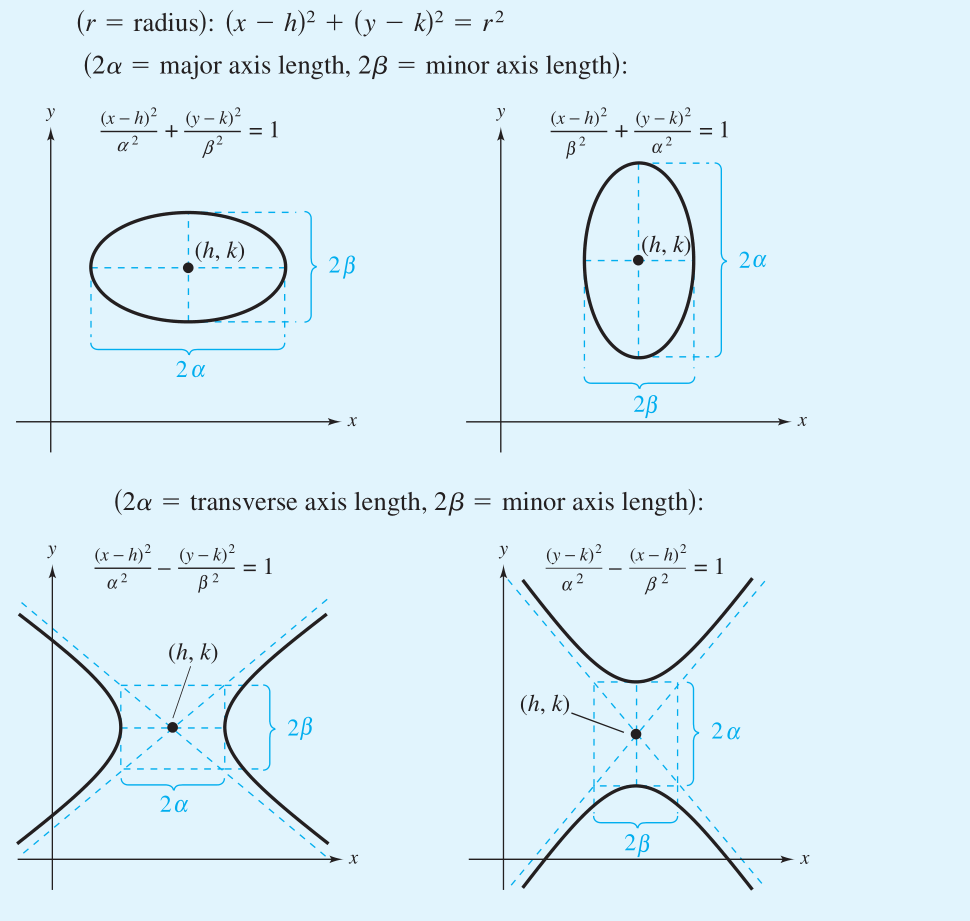
\includegraphics[width = 13cm]{images/coniceq.png} \\
        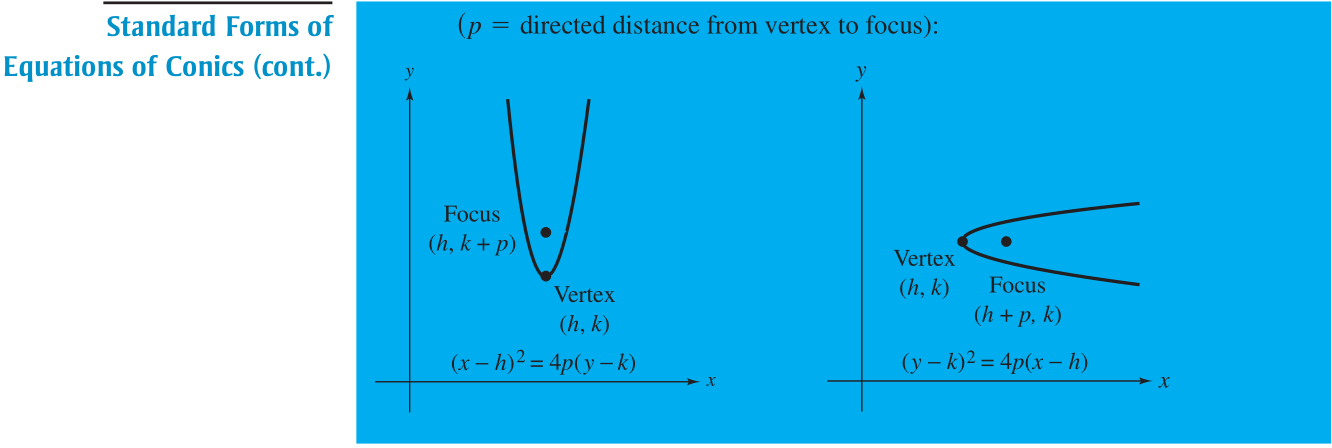
\includegraphics[width = 16cm]{images/conic1.png}
    \end{center}

    For a second-degree polynomial equations that have an $xy$-term, the axes are not \T{parallel} to the coordinate
    axes. In such cases, it is helpful to \T{rotate} the standard axes to form the new $x'$-axis and $y'$-axis.

    The required rotation angle $\theta$ (measure counterclockwise) is $\cot{2\theta} = (a - c)/b$. With this rotation, 
    the standard basis in the plane
    \[ B = \{ (1,0), (0,1) \} \]
    is rotated to form the new basis
    \[ B' = \{ (\cos{\theta}, \sin{\theta}), (-\sin{\theta}, \cos{\theta})\]
    \begin{center}
        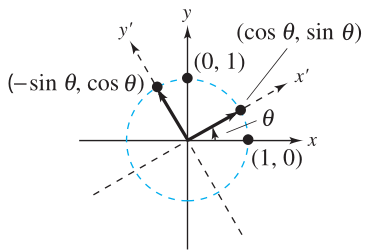
\includegraphics[width = 5cm]{images/rotateaxes.png}
    \end{center}
    To find the coordinates of $(x,y)$ relative to this new basis, use a \T{transition matrix}.

    \subsection{A Transition Matrix for Rotation in the Plane}
    Find the coordinate of  a point $(x,y)$ in $R^2$ relative to the basis 
    \[ B' = \{ (\cos{\theta}, \sin{\theta}), (-\sin{\theta}, \cos{\theta})\} \]

    \T{SOLUTION.} By Theorem 4.21, you have
    \[ [B' \vdots B] = 
        \begin{bmatrix}
            \cos{\theta} & -\sin{\theta} & \vdots & 1 & 0 \\
            \sin{\theta} & \cos{\theta} & \vdots & 0 &  1
        \end{bmatrix} \]
    \[ \begin{bmatrix}
        I & \vdots & P^{-1}
    \end{bmatrix} = 
    \begin{bmatrix}
        1  & 0 & \vdots & \cos{\theta} & \sin{\theta} \\
        0 & 1 & \vdots & -\sin{\theta} & \cos{\theta}
    \end{bmatrix} \]
    The $x'$- and $y'$- coordinates are 
    \[\begin{cases} 
        x' = x \cos{\theta} + y\cos{\theta}\\
        y' = -x\sin{\theta} + y\cos{\theta}
    \end{cases}\]
    It is also important to express the $xy$-coordinates in terms of the $x'y'$-coordinates. 
    \[ x = x'\cos{\theta} - y'\sin{\theta} \quad \text{ and  } \quad y = x'\sin{\theta} + y'\cos{\theta}\]
    Substituting these expressions for $x$ and $y$ into the given second-degree equation produces
    a second-degree polynomial equation in $x'$ and $y'$ that has no $x'y'$-term.

    \tcl
    \B{Rotation of Axes.}
        The second-degree equation $ax^2 + bxy + cy^2 + dx + ey + f = 0$ can be written in the form
        \[ a'(x')^2 + c'(y')^2 + d'x' + e'y' + f' = 0 \]
        by rotating the coordinates axes counterclockwise through the angle $\theta$, where $\theta$ is defined by
        $\cot{2\theta} = \frac{a - c}{b}$. The coefficients of the new equation are obtained from
        the substitutions
        \[ \begin{cases}{}
            x = x'\cos{\theta} - y'\sin{\theta} \\
            y = x'\sin{\theta} + y'\cos{\theta}
        \end{cases} \]
    \etcl 











    




\end{document}
